% !TEX root = trkjet.tex

\part*{Auxiliary material}
\addcontentsline{toc}{part}{Auxiliary material}
%-------------------------------------------------------------------------------

%In an ATLAS paper, auxiliary plots and tables that are supposed to be made public 
%should be collected in an appendix that has the title \enquote{Auxiliary material}.
%This information will appear on the public webpage, but will not be included
%in the document submitted to arXiv and to the journal.


\begin{figure}[h]
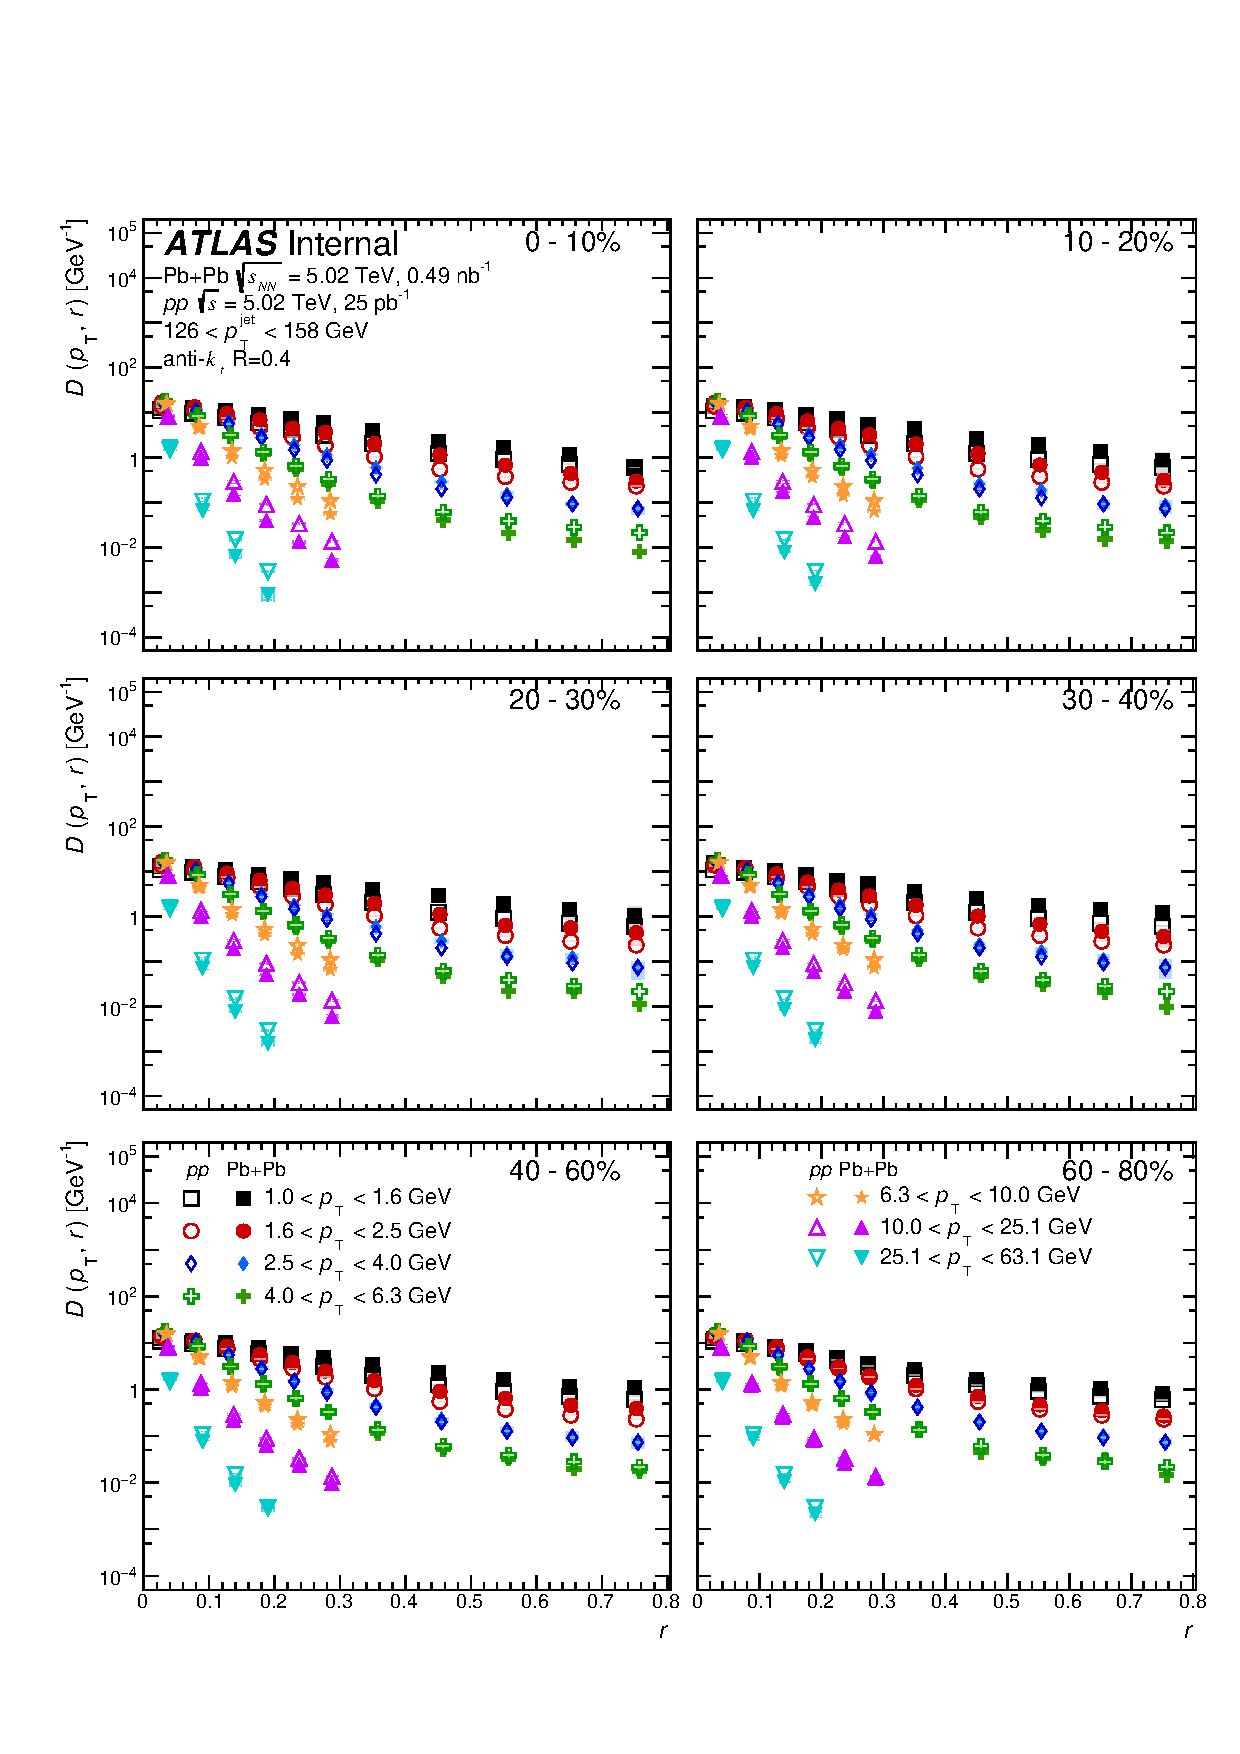
\includegraphics[width=1.0\textwidth]{figures/results/DpT_dR_jet7.pdf}
\caption{Full set of \Dptr\ distributions for 126--158 GeV jets.}
\label{fig:fullset_dptr_j7}
\end{figure}

\begin{figure}[h]
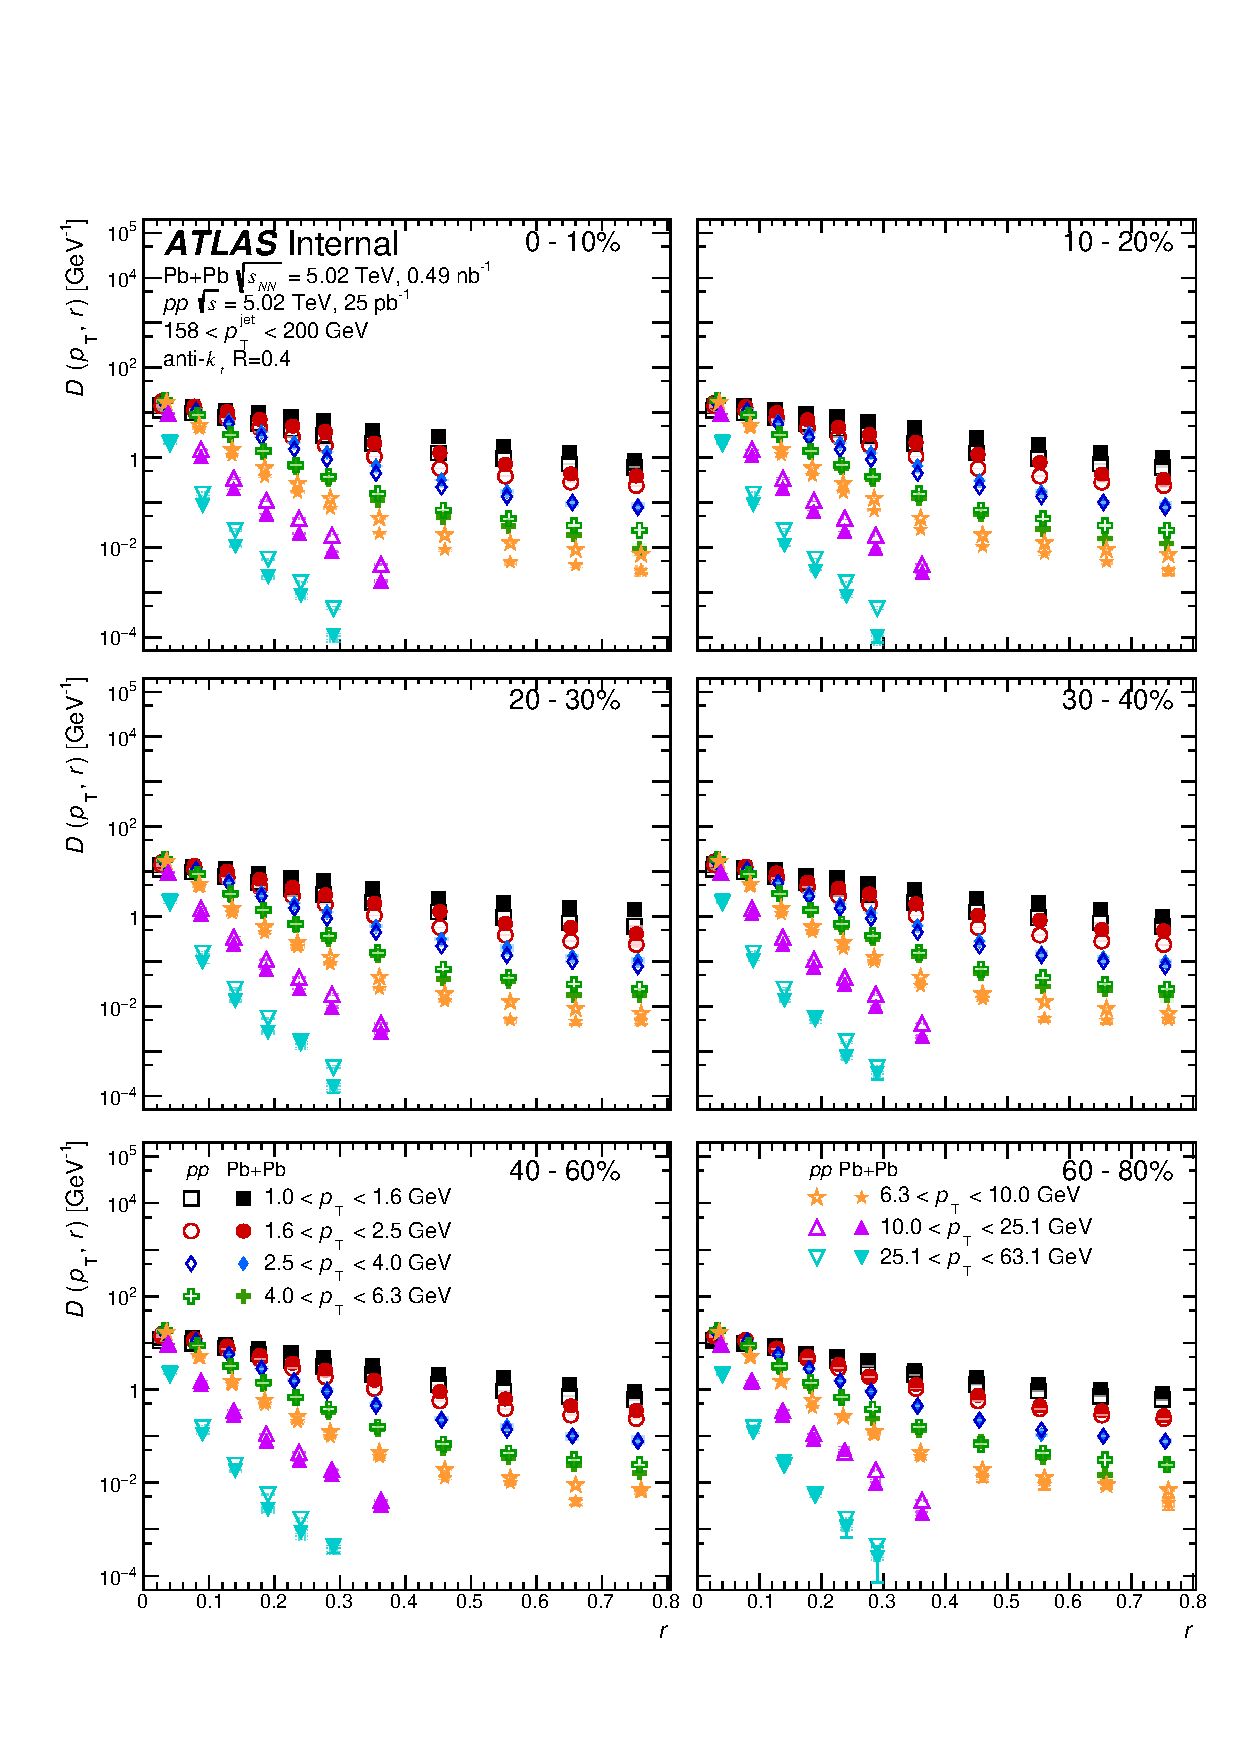
\includegraphics[width=1.0\textwidth]{figures/results/DpT_dR_jet8.pdf}
\caption{Full set of \Dptr\ distributions for 158--200 GeV jets.}
\label{fig:fullset_dptr_j8}
\end{figure}

\begin{figure}[h]
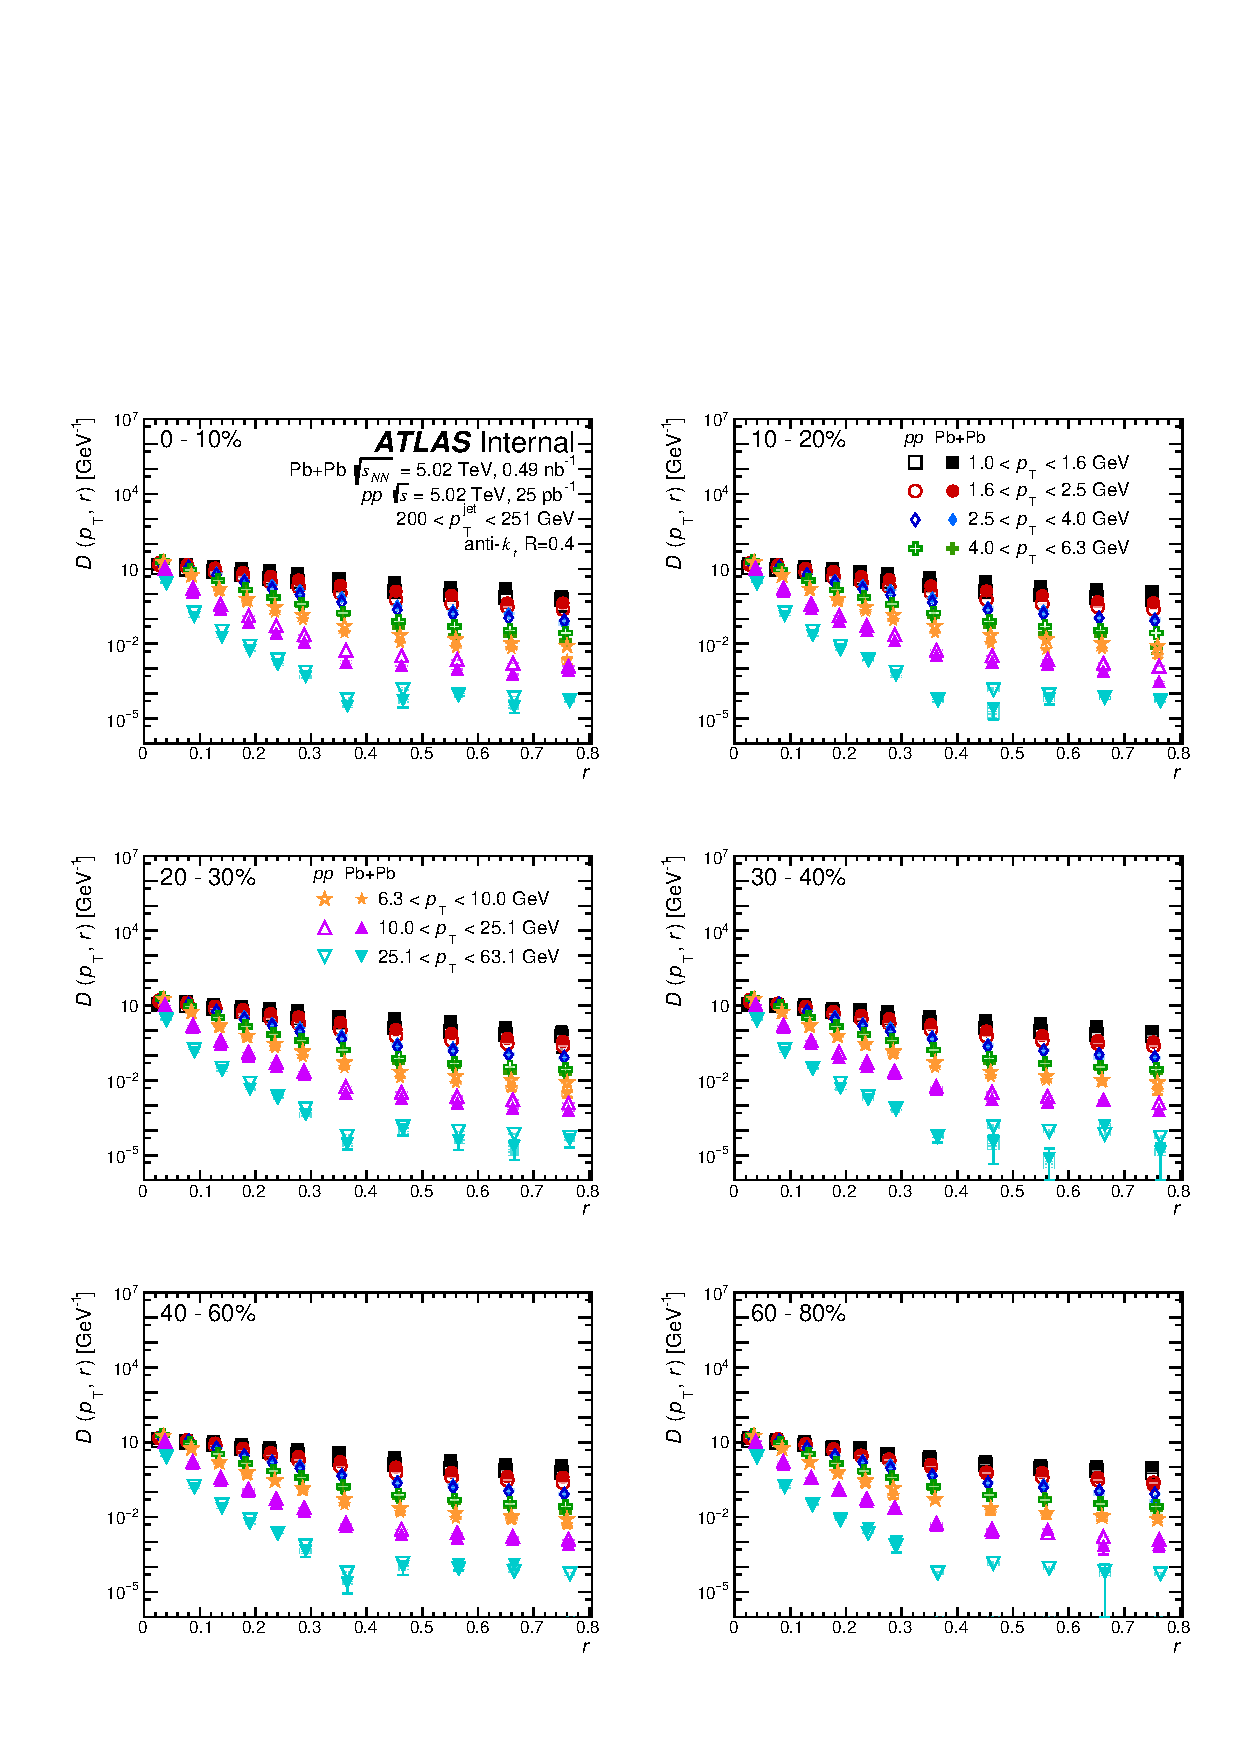
\includegraphics[width=1.0\textwidth]{figures/results/DpT_dR_jet9.pdf}
\caption{Full set of \Dptr\ distributions for 200--251 GeV jets.}
\label{fig:fullset_dptr_j9}
\end{figure}

\begin{figure}[h]
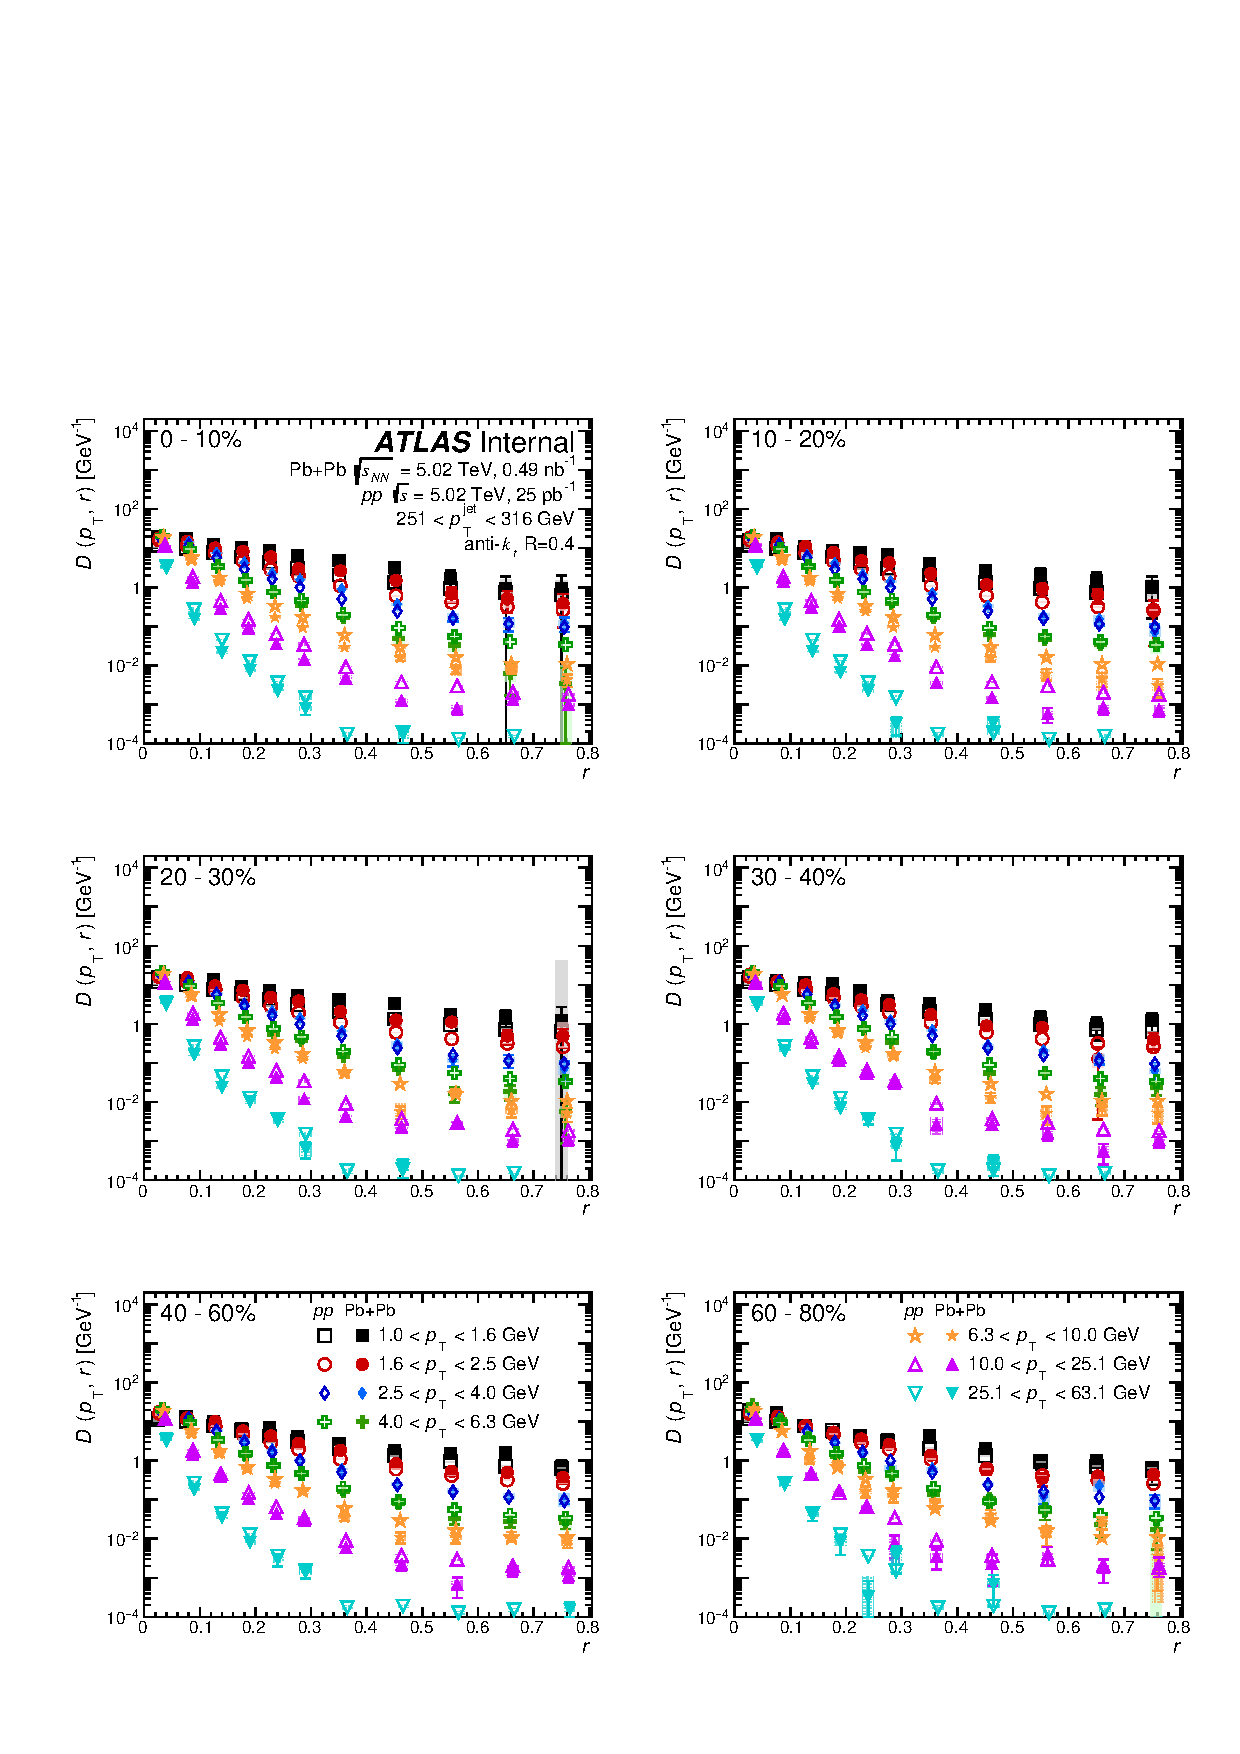
\includegraphics[width=1.0\textwidth]{figures/results/DpT_dR_jet10.pdf}
\caption{Full set of \Dptr\ distributions for 251--316 GeV jets.}
\label{fig:fullset_dptr_j10}
\end{figure}


\begin{figure}[h]
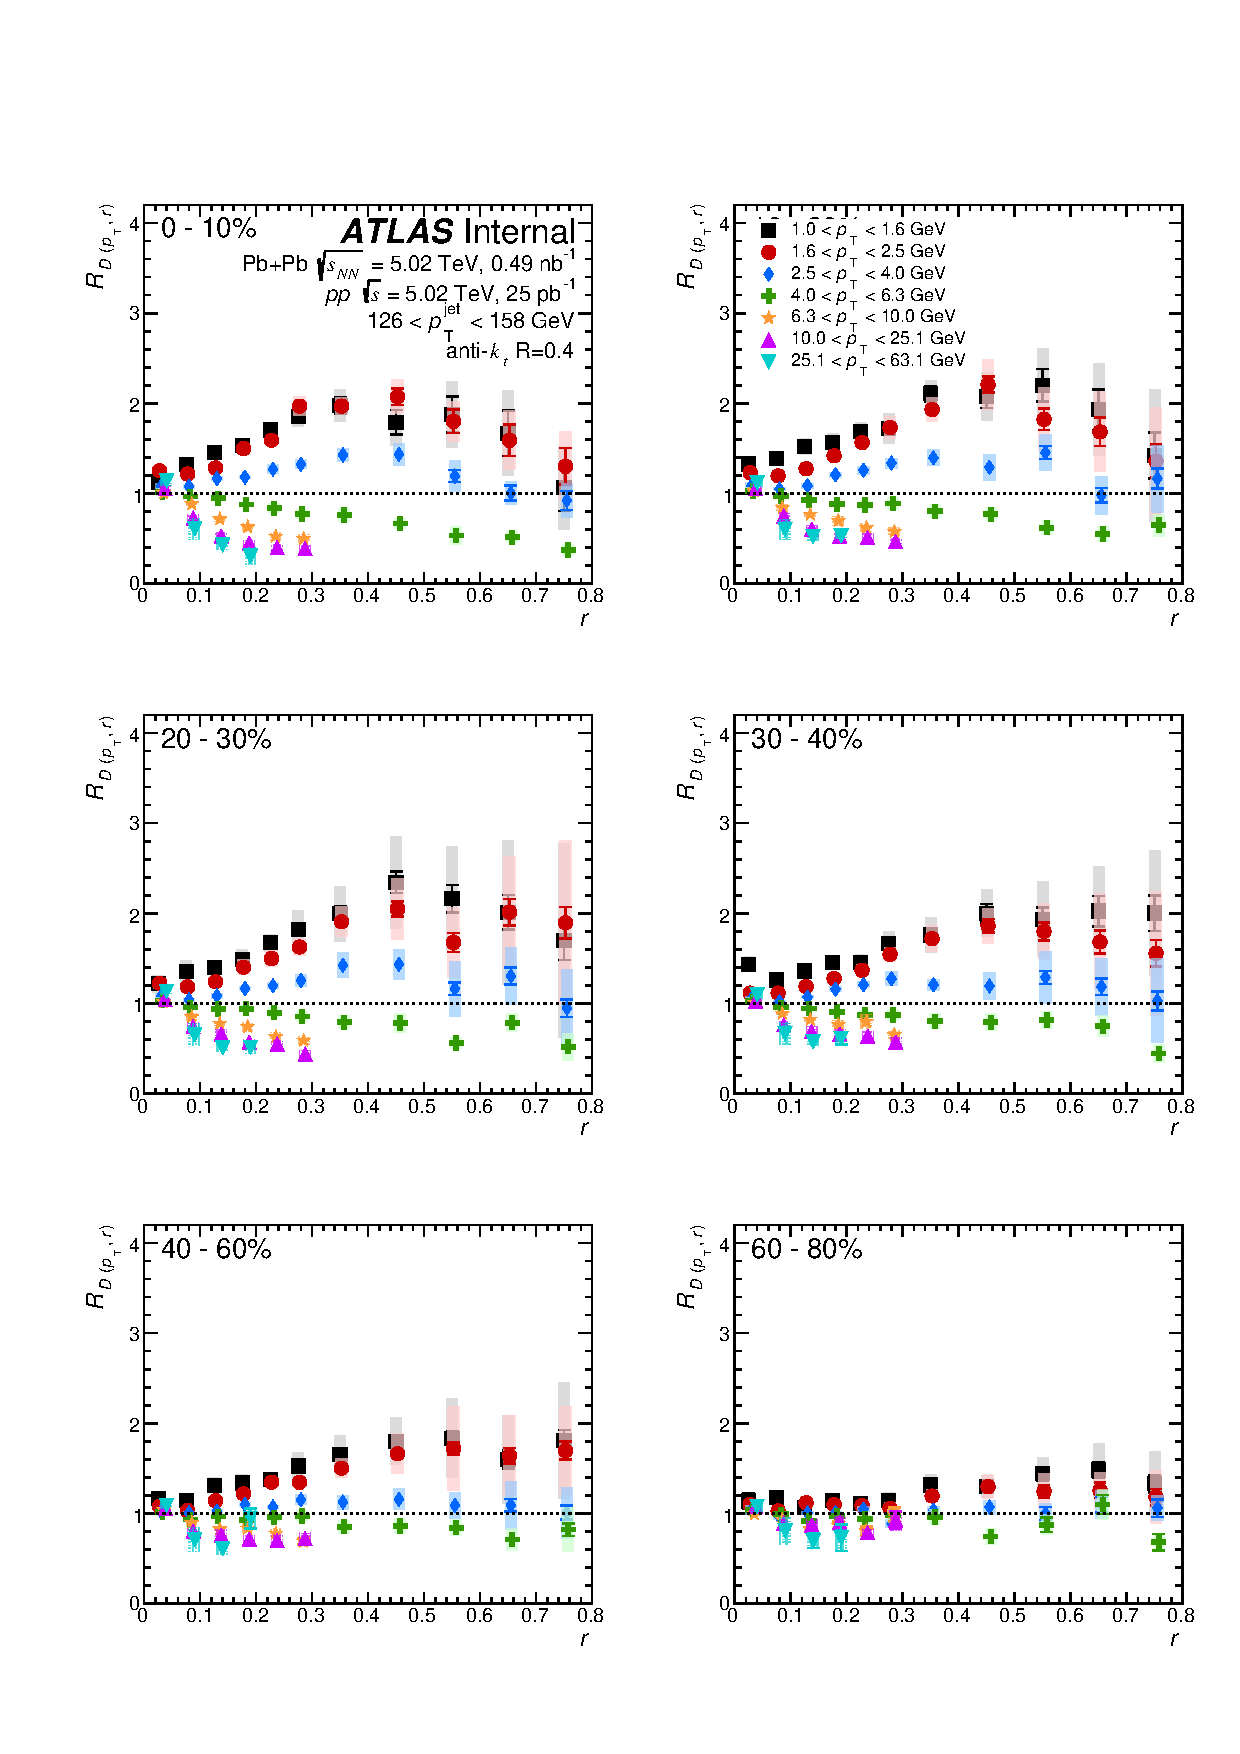
\includegraphics[width=1.0\textwidth]{figures/results/RDpT_dR_jet7.pdf}
\caption{Full set of \RDptr\ distributions for 126--158 GeV jets.}
\label{fig:fullset_rptr_j7}
\end{figure}

\begin{figure}[h]
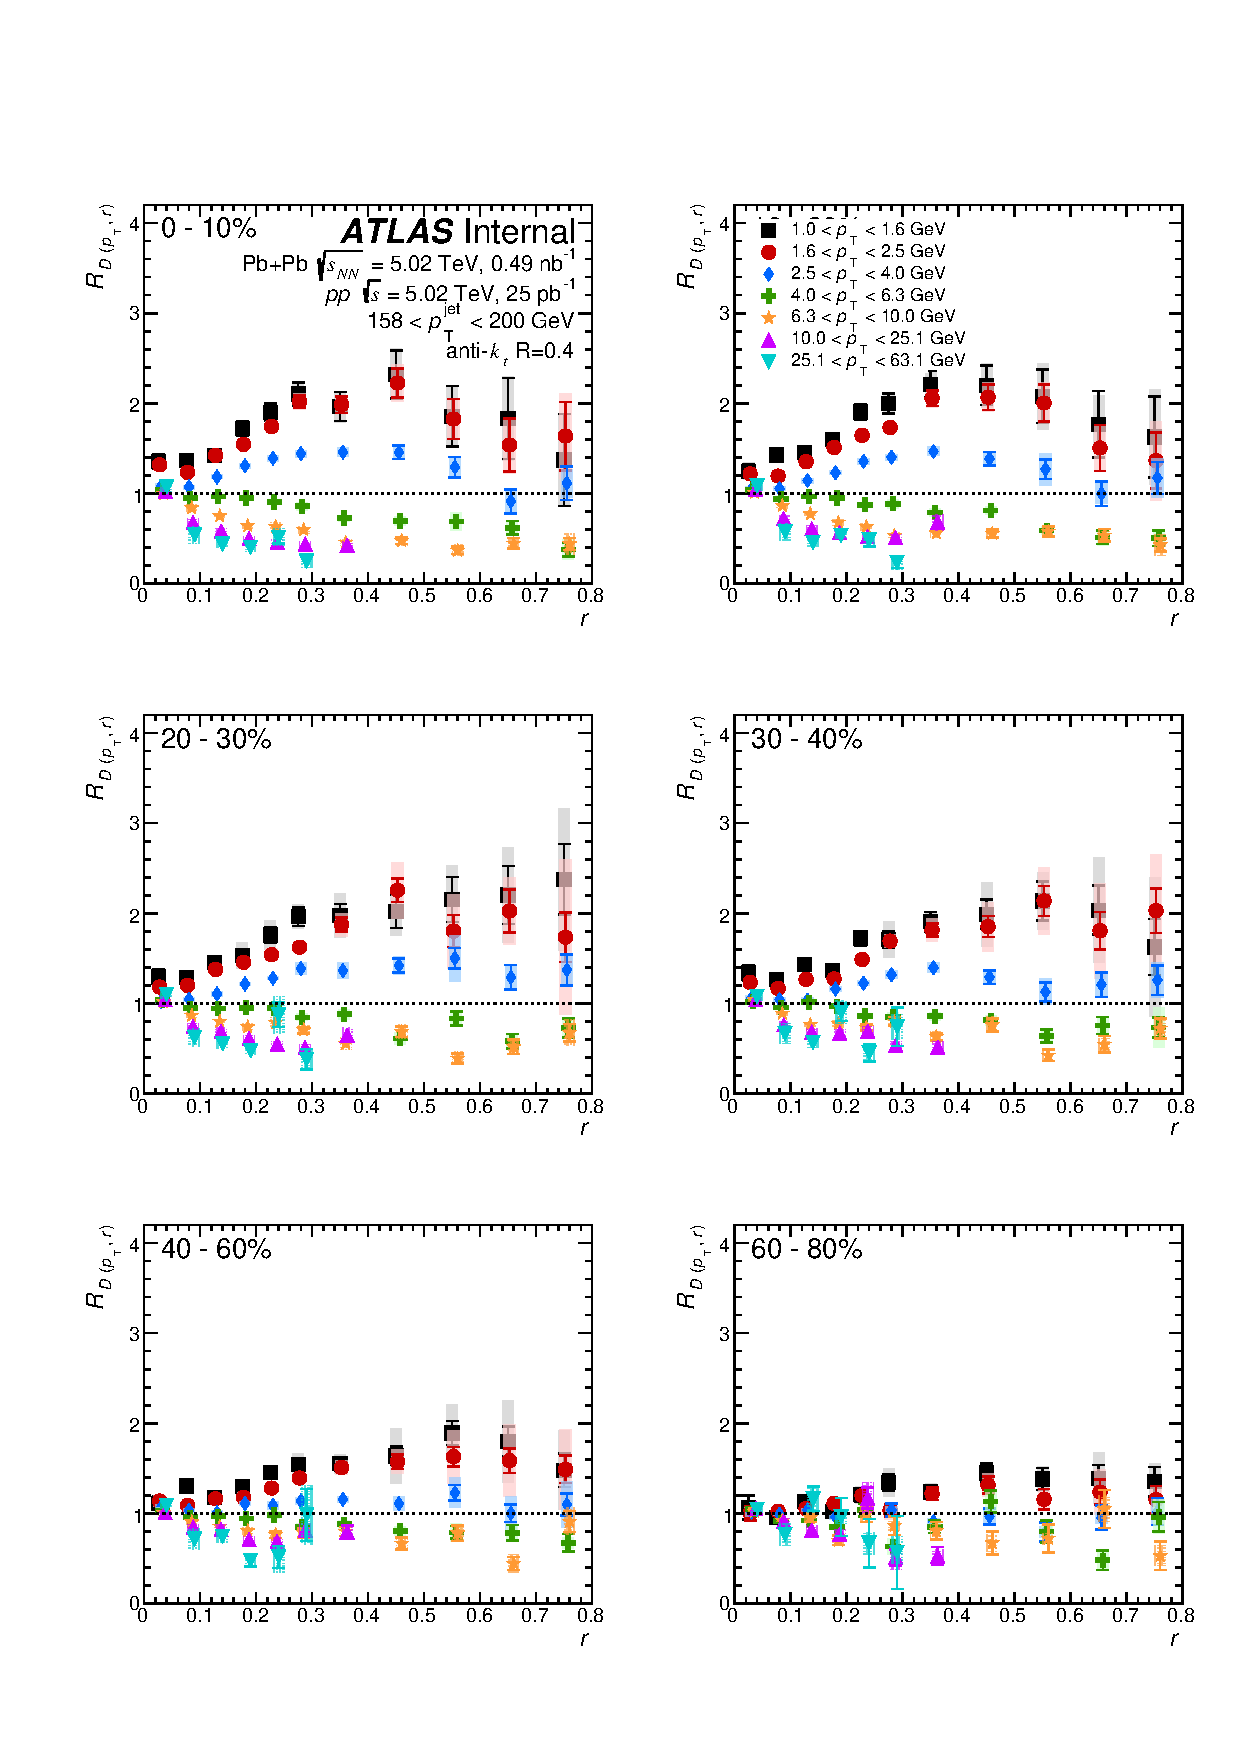
\includegraphics[width=1.0\textwidth]{figures/results/RDpT_dR_jet8.pdf}
\caption{Full set of \RDptr\ distributions for 158--200 GeV jets.}
\label{fig:fullset_rptr_j8}
\end{figure}

\begin{figure}[h]
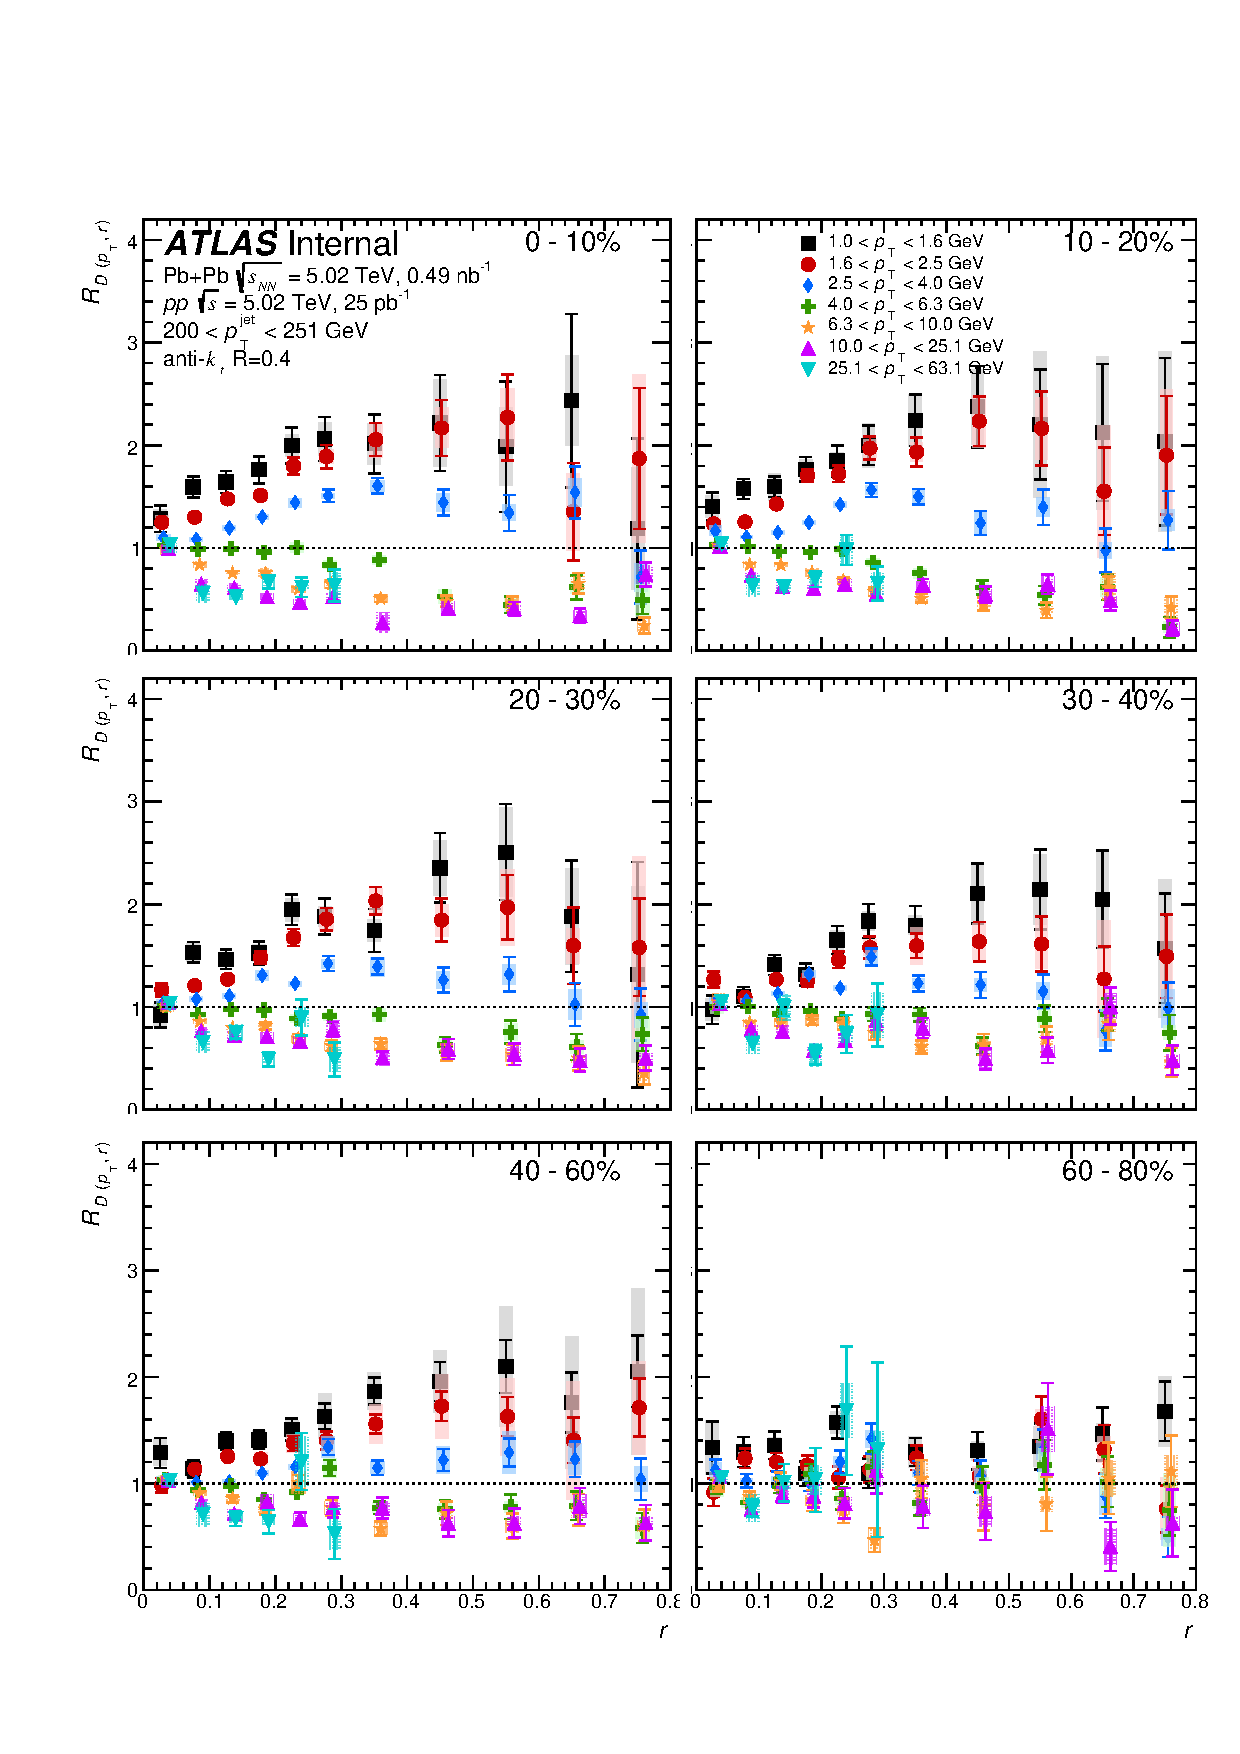
\includegraphics[width=1.0\textwidth]{figures/results/RDpT_dR_jet9.pdf}
\caption{Full set of \RDptr\ distributions for 200--251 GeV jets.}
\label{fig:fullset_rptr_j9}
\end{figure}

\begin{figure}[h]
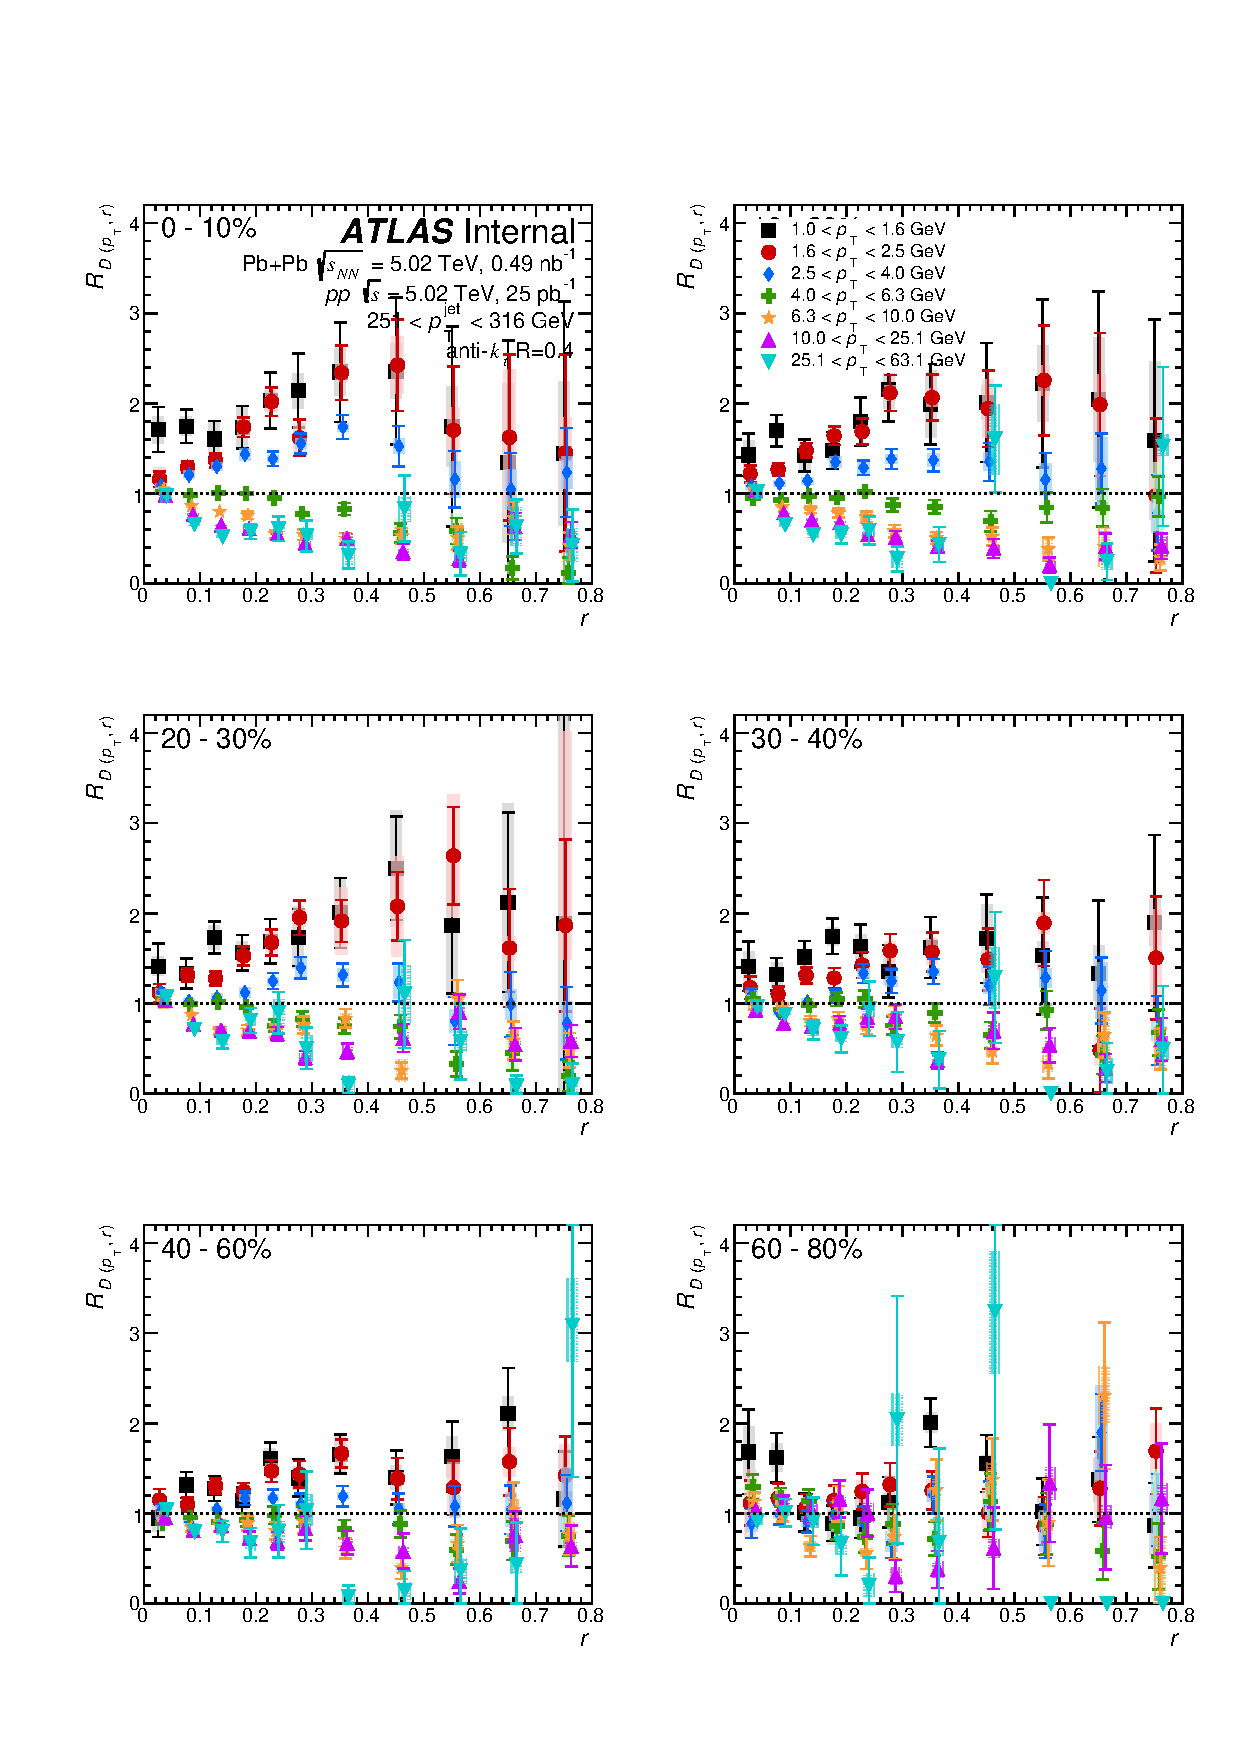
\includegraphics[width=1.0\textwidth]{figures/results/RDpT_dR_jet10.pdf}
\caption{Full set of \RDptr\ distributions for 251--316 GeV jets.}
\label{fig:fullset_drtr_j10}
\end{figure}
